\documentclass[12pt]{article}
\usepackage[margin=0.75in]{geometry}
\geometry{a4paper}
\usepackage[T1]{fontenc} % Support Icelandic Characters
\usepackage[utf8]{inputenc} % Support Icelandic Characters
\usepackage{graphicx} % Support for including images
\usepackage{hyperref} % Support for hyperlinks
\usepackage{wrapfig}

\usepackage{algorithm}
\usepackage{algorithmicx}
\usepackage{listings}
\usepackage{color}
\usepackage{siunitx}

\usepackage[svgnames]{xcolor}

\usepackage{amsmath}
\usepackage{tikz}
\usetikzlibrary{arrows,automata}

\usepackage{tikz}
\usepackage{tikz-dependency}
\usepackage[spanish,es-noshorthands]{babel}

\usepackage[spanish]{babel}
\usepackage[latin1]{inputenc}
\usepackage[usenames]{color}

\definecolor{mGreen}{rgb}{0,0.6,0}
\definecolor{mGray}{rgb}{0.5,0.5,0.5}
\definecolor{mPurple}{rgb}{0.58,0,0.82}
\definecolor{backgroundColour}{rgb}{0.95,0.95,0.92}

\usepackage{xcolor}

\usepackage{listings}             % Include the listings-package
\lstdefinestyle{CStyle}{
    backgroundcolor=\color{backgroundColour},   
    commentstyle=\color{mGreen},
    keywordstyle=\color{blue},
    numberstyle=\tiny\color{mGray},
    stringstyle=\color{red},
    basicstyle=\footnotesize,
    breakatwhitespace=false,         
    breaklines=true,                 
    captionpos=b,                    
    keepspaces=true,                 
    numbers=left,                    
    numbersep=5pt,                  
    showspaces=false,                
    showstringspaces=false,
    showtabs=false,                  
    tabsize=2,
    language=C
}



%------------------------------------------------------------------
% TITLE
%------------------------------------------------------------------

\title{
\centerline{
    
\includegraphics[width=75mm]{unsa.png}}
    \vspace{0.5 cm}
        Teoría de la Computación - Laboratorio A
        \\
        \\
        \\
        \textbf{Práctica de Laboratorio #7} 
        \large  
        \\
        %SC-T-718-ATSR,Automatic Speech Recognition, 2019-1 
        %\\ 
        \small Universidad Nacional de San Agustín - Escuela Profesional de Ingeniería de Sistemas, Arequipa, Perú 
  }

\author{
    Carlos Alberto Mestas Escarcena
    \\
    \texttt{cmestas@unsa.edu.pe}
}

\date{Junio del 2020}

\begin{document}

\maketitle

El desarrollo de este informe se puede encontrar en el repositorio de \textcolor{blue}{
    \href{https://github.com/CarlosMestas/TC_A_6_Carlos_Mestas}{GitHub}}.

\section{La construcción While es ambigua?}
    Sería no ambigua ya que tiene solamente una manera correcta de como interpretarse.
    
\begin{figure}[h]
    \centering
    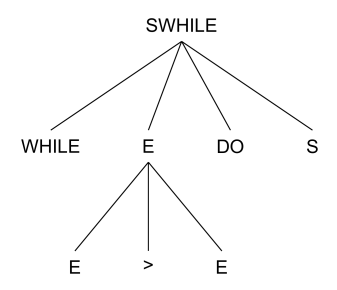
\includegraphics[width=0.25\textwidth]{images/While.PNG}
    \caption{While}
\end{figure}
    
    


\section{Implementar las llaves para limitar el ámbito de un programa}

\begin{lstlisting}[language=bash,frame=single,style=CStyle,caption={lexico.l}]
%{
    #include "sintactico.tab.h"

%}
number [0-9]+
%%
{number}            {yylval = atoi(yytext);
                     return (NUM);}
\n                  {return (EOL);}
.                   {return yytext[0];}
%%
int yywrap(){
    return 0;
}
\end{lstlisting}

\begin{lstlisting}[language=bash,frame=single,style=CStyle,caption={sintactico.y}]
%{
    #include <stdio.h>
    #include <stdlib.h>
    extern int yylex();
    extern char *yytext;
    void yyerror(char* s);

%}
%token NUM
%token EOL

%left '+' '-'
%left '*' '/'

%%
stm_lst: stm stm_lst EOL 
       | stm EOL 
       ;

stm: exp        {printf("= %d \n",$1);
                exit(0);}
   ;

exp: exp '+' exp   { $$= $1 + $3;}
   | exp '-' exp   { $$= $1 - $3;}
   | exp '*' exp   { $$= $1 * $3;} 
   | exp '/' exp   { 
                      if($3!=0){
                        $$= $1 / $3;
                        }
                      else{
                        yyerror("No hay division entre 0");
                        $$ = 0;
                      }
                    }
   |  '{' exp '}'   { $$= $2;}
   |  '(' exp ')'   { $$= $2;}
   |  NUM           { $$= $1;}
   ;
%%

void yyerror(char* s){
    printf(" Error sintactico: %s \n",s);
}

int main(int argc,char **argv){
    yyparse();
    return 0;
}
\end{lstlisting}

\begin{figure}[h]
    \centering
    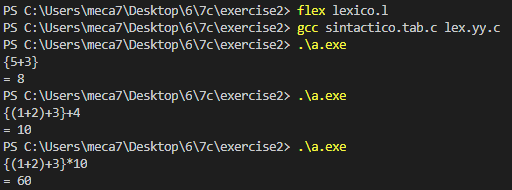
\includegraphics[width=0.6\textwidth]{images/Capture002A.PNG}
    \caption{Ejecución - Ejercicio 2}
\end{figure}

\section{Quitar la ambigüedad al ejercicio 17}

\begin{lstlisting}[language=bash,frame=single,style=CStyle,caption={lexico.l}]
%{
    #include "sintactico.tab.h"
%}
number [0-9]+
variable [a-zA-Z]+
%%
{number}                {return (NUM);}
{variable}              {return (VAR);}
"+"                     {return (SYMBOLSUM);}
"\n"                    {return (EOL);}
.                       {return yytext[0];}
%%
int yywrap(){
    return 0;
}
\end{lstlisting}

\begin{lstlisting}[language=bash,frame=single,style=CStyle,caption={sintactico.y}]
%{
    #include <stdio.h>
    #include <stdlib.h>
    extern int yylex();
    extern char *yytext;
    void yyerror(char* s);

%}
%token NUM
%token VAR
%token SYMBOLSUM
%token EOL

%left SYMBOLSUM
%%

s: expcad EOL                   
 | expnum EOL                       
 | expcad SYMBOLSUM expnum      {printf("Se reconocio una una suma de variables mas numeros \n");}
 | expnum SYMBOLSUM expcad      {printf("Se reconocio una de numeros mas variables \n");}
 ;

expcad: expcad SYMBOLSUM expcad {printf("Se reconocio una suma de variables \n");}
      | '(' expcad ')'
      | VAR
      ; 

expnum: expnum SYMBOLSUM expnum {printf("Se reconocio una suma de numeros \n");} 
      | '(' expnum ')'
      | NUM
      ; 

%%

void yyerror(char* s){
    printf(" Error sintactico: %s \n",s);
}

int main(int argc,char **argv){
    yyparse();
    return 0;
}
\end{lstlisting}

\begin{figure}[h]
    \centering
    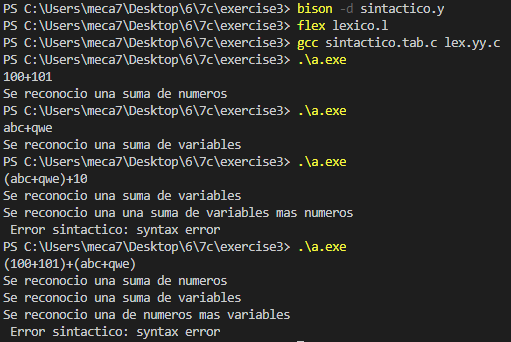
\includegraphics[width=0.6\textwidth]{images/Capture003A.PNG}
    \caption{Ejecución - Ejercicio 3}
\end{figure}

\clearpage
\newpage

\end{document}